\documentclass[fleqn,10pt]{wlscirep}
\title{Whole Genome Alignment And Comparative Annotation}
\usepackage{indentfirst}
\usepackage{amssymb}
\author[1,*]{Joel Armstrong}
\author[1,*]{Ian Fiddes}
\author[1,]{Mark Diekhans}
\author[1,+]{Benedict Paten}
\affil[1]{Genomics Institute, University of California Santa Cruz and Howard Hughes Medical Institute, Santa Cruz, CA 95064, USA}

\affil[+]{Corresponding author. Email: bpaten@ucsc.edu}

\affil[*]{these authors contributed equally to this work}

%\keywords{Keyword1, Keyword2, Keyword3}

\begin{abstract}
TBA
\end{abstract}
\begin{document}

\flushbottom
\maketitle

\thispagestyle{empty}

\section{Whole-genome alignments}
\subsection{Introduction}
Alignment is possibly the most fundamental problem in genomics.
The alignment problem is to establish a mapping between the letters of a set of sequences that approximates some relation that the user is interested in.
In comparative genomics, we are generally interested in the \emph{homology} relation---that is, does the lineage of two bases coalesce at a single base in a single organism at some point in time?
In typical real-world comparative genomics, there is no clear proof of homology, as we have absolutely no access to the true history of every base in a set of sequences.
However, we can use our knowledge of molecular evolution to construct very good approximations to the homology relation.
The potential for using sequence similarity to approximate homology was recognized and applied very early on, starting with the pioneering work of Needleman and Wunsch on optimal pairwise global alignment~\cite{Needleman1970443}.
The pairwise global alignment work was quickly specialized to perform \emph{local alignment}, which calculates the optimal alignment of subsequences rather than sequences, by Smith and Waterman~\cite{Smith1981}.

The \emph{whole-genome alignment} problem involves aligning two or more genomes, or other large sequences or set of sequences, together.
While whole-genome alignment is essentially just alignment writ large, it is generally treated differently than short sequence alignment because two factors not usually considered in short alignments become impossible to ignore: size and rearrangements.
The size of the problem in whole-genome alignment causes alignments to take too long to be practical, forcing efficiency considerations to be taken into account.
The traditional dynamic-programming algorithms require $O(nm)$ time and space, where $n$ and $m$ are the lengths of the two sequences; obviously, as $n$ and $m$ grow to genome-scale the problem becomes too expensive to solve in practice.
Another consideration is how genome rearrangements complicate the alignment problem.
Smith-Waterman and Needleman-Wunsch both produce alignments which have \emph{fixed order-and-orientation}, that is, insertions, deletions, and substitutions are the only allowed edit operations.
When looking at short or well-conserved sequences, like genes, this requirement is usually fulfilled.
But at large evolutionary distances, genomes almost always contain more complex rearrangements with respect to each other---inversions, transpositions, and duplications all cause breaks in order and orientation that cannot be captured under constant order and orientation.

One obvious solution to these problems is to use a fast approximate local alignment algorithm (like BLAST~\cite{blast}) and simply use the collection of all local alignments that it finds as the whole-genome alignment.
However, the naïve local alignment approach has its own problems.
Whole-genome local alignments have both too low sensitivity and too low specificity to be useful at substantial evolutionary distances.
That is, local alignments will miss homologous sequence that, by chance, happened to be further diverged.
They will also capture spurious alignments that can obscure the more useful data.
Even when they correctly identify homologous regions, the end-user is more often interested in \emph{orthology} rather than homology: ancient duplications may share similar sequence, but often do not share similar function.
We call any alignment that allows rearrangements (i.e.\ does not have fixed order-and-orientation) and attempts to determine orthology rather than just homology (even if restricted to single-copy) a \emph{whole-genome alignment} (or for short, a \emph{genome alignment}).
Most whole-genome alignment methods are based on local alignments, but do some filtering and post-processing to construct a useful end product~\cite{Batzoglou2005}.

As long DNA sequences became available, it was soon recognized that Needleman-Wunsch or Smith-Waterman alignments were far too slow to be useful for megabase-scale sequences, much less chromosome-scale sequences.
The impractical running time of global alignment drove the development of several tools~\cite{avid,mummer,lagan} that produce an approximately optimal global alignment through the use of high-confidence \emph{anchors} in a single order and orientation, which are then used to partition the alignment into smaller problems which can be more efficiently solved.
These anchors provided a very efficient and reliable way to break up the alignment problem, but relied on a constant order and orientation, which excluded any possibility of noticing rearrangements.

\emph{Chaining}~\cite{evoCauldron} is a powerful technique for making sense of pairwise local alignments.
Chains are simply maximal combinations of local alignments that maintain a single order and orientation.
Chaining provides a good way of filtering out spurious alignments, which are likely to form short, low-scoring chains.
However, the set of chains can often include distant paralogs or spurious sequence, which makes it difficult to understand the rearrangements that have taken place between the two input genomes.
\emph{Netting}~\cite{evoCauldron} is a related technique that makes rearrangements relative to a reference genome much easier to find.
In essence, netting finds the best-scoring set of chains that covers the bases of the reference genome only once.
This makes it very easy to find high-confidence rearrangements like transpositions, inversions, and deletions, but throws away the effect of duplications in the target genome.


Choosing the single ``best'' target alignment for each region, which we will call the \emph{single-copy} strategy, is a common way~\cite{blastz,tba} to deal with the problems that duplications cause.
However, the best-fit strategy will not always find a correct ortholog, and indeed even reciprocally-best-fit is not enough to guarantee finding an ortholog~\cite{recipBestOrtholog}.
But most importantly, lineage-specific duplications should not be ignored.
When lineage-specific duplication occurs, a gene outside that lineage will have \emph{multiple} orthologs in the lineage, and should be aligned to multiple copies~\cite{Koonin2005}.
Single-copy alignments implicitly assume that orthology is a one-to-one relationship.
However, in nature, orthology is a many-to-many relationship~\cite{Koonin2005}.
When that assumption of one-to-one orthology is violated, single-copy alignments can be very misleading.

\subsection{Multiple alignment}
Often it is necessary to consider the alignment between a set of more than two sequences, which we call \emph{multiple alignment}.
A multiple alignment is defined as an equivalence relation $\sim$ on a set of sequences $\mathcal{S} = \{s_1, s_2, \ldots\}$, such that for two bases $b_1 \in s_1 \in \mathcal{S}$ and $b_2 \in s_2 \in \mathcal{S}$, $b_1 \sim b_2$ if they are considered to be aligned to each other.
The alignment is partitioned into \emph{columns} by the equivalence classes of $\sim$: i.e.\ every base is related to all bases in its column, and no two bases in different columns are related.

Unfortunately, multiple alignment is a significantly more difficult problem than pairwise alignment.
Finding an optimal multiple alignment, even using very simple objective functions, has long been known to be NP-hard~\cite{complexityOfMultipleAlignment}.
Heuristics must be employed to efficiently solve the multiple alignment problem.

\emph{Progressive alignment} is the most popular strategy for approximate multiple alignment~\cite{progressiveAlignment}.
Progressive alignment uses as an additional input a \emph{guide tree} relating the input sequences.
The most closely related sequences are aligned first, then the resulting alignment is itself aligned to other sequences or alignments, following the structure of the guide tree. Often consensus sequences are used as a method of aligning alignments.

Since the multiple alignment problem is so difficult, another approach is to use a single \emph{reference} sequence to base the alignment on.
All other sequences in the multiple alignment are simply aligned to this genome in a pairwise fashion, then the several pairwise alignments are combined to form a \emph{reference-biased} multiple alignment.
This approach performs very well when viewed from the reference genome, but information relating genomes distant from the reference is lost. See \ref{fig:referencefree} for an illustration of this effect.

In the mid- to late-2000s the first methods for reference-free multiple genome alignment allowing multiple copies began to appear (notably the Enredo-Pecan-Ortheus (EPO) pipeline~\cite{epo} and the A-Bruijn aligner~\cite{aBruijn}).
The EPO pipeline especially began to see wide use as part of the Ensembl genome browser~\cite{ensembl2017}.
While impressive, these pipelines left significant room for improvement, especially with regard to finding small-scale order-and-orientation-breaking rearrangements~\cite{epo}.

\subsection{Reference-free alignment}
\subsubsection{Genome histories}
Alignments are conventionally described as a set of columns, each containing a set of bases that are all related to each other by some alignment relation $\sim$.
Usually this relation represents orthology rather than homology.
However, in that case, this model falls apart when considering reference-free alignments with multiple copies per genome.
The orthology relation is not transitively closed~\cite{Koonin2005}, so it is impossible in the general case to create a set of columns containing bases that are all orthologous to each other.
The only way to represent a reference-free, multi-copy, orthologous multiple genome alignment is by associating the alignment with phylogenetic trees, which are inferred (even if implicitly) during the alignment process.
We term these types of alignments \emph{genome histories} to reflect that they require a different representation than typical alignments (which can be represented by a collection of only blocks or columns).

A \emph{genome history} $\{\mathcal{S}, \sim, T_c, t_s, L\}$ consists of a set of genomes $\mathcal{S}$, a multiple alignment $\sim$ relating the bases of those genomes, a reconciled tree $t \in T_c$ for each column in that alignment, a species tree $t_s$, and, optionally, a set of \emph{links} $L$ between columns, indicating the ordering of the ancestral chromosomes.
The columns of the genome history reflect the \emph{homology} rather than \emph{orthology} relation.
Since homology is transitive, the homology-based alignment can be represented by columns.
The set of trees (hereafter referred to as \emph{column trees}) indicate the evolutionary history of the bases in each column.
Where there are duplications, gains, or losses, the column tree $t \in T_c$ will differ from the species tree $t_s$.
Though the genome history representation we present here is not the only possible representation, any other representation (such as a collection of all pairwise orthology relationships) can be transformed into this one.

A genome history can be used to define both \emph{orthology} and \emph{paralogy} relations.
The orthology relation, which we will symbolize by $\sim_o$, uses the column trees of the genome history to determine which of the homologous bases in a column are also orthologous to each other.
The orthologous bases are those homologous bases whose lineage coalesces in a speciation event in the column tree~\cite{Koonin2005}.
The paralogy relation $\sim_p$ simply relates homologous bases which are not orthologs.

A genome history can be \emph{projected} onto any genome to create a more conventional referenced multiple alignment.
These projected, reference-based alignments are collections of columns, each containing exactly one reference base, where every base in the column is orthologous to the reference base, but \emph{not} necessarily orthologous to every other base in the column.
These projected alignments are useful because they can be represented in conventional formats like MAF, and used as input to existing analysis tools.

\subsubsection{HAL format}
% TODO(joel): this is underselling it a bit. The key point here---one that I don't think is actually brought up properly anywhere in the literature---is that block formats like MAF are not only inefficient for reference-free alignments, they fundamentally can't represent them without additional information (like column/block trees).
One difficulty with producing reference-free alignments is that conventional text-based alignment formats like MAF cannot be efficiently randomly accessed from every genome. The Hierarchical Alignment Format~\cite{hal} (HAL) was designed to be an efficiently accessible format representing a genome history, including any ancestral reconstructions available.

HAL allows projection from this genome history onto any reference genome (including ancestors), creating a multiple genome alignment showing what is orthologous (related by $\sim_o$) to every base in that genome. This projection can be output in a traditional format like MAF, or simply used on-demand to visualize the alignment~\cite{assemblyHub} or as part of downstream analysis pipelines.
% \subsection{Local alignment tools}
% don't think much detail about local alignment really belongs in a paper about genome alignment. Maybe worth a quick mention?
\subsection{Multiple genome alignment pipelines}
\subsubsection{MultiZ}
MultiZ~\cite{tba} is a reference-biased multiple genome alignment tool originally developed as part of the TBA~\cite{tba} program.
% TODO(joel): might need to come up with a citation here to justify that pretty much no one uses TBA.
% TODO(joel): there is supposedly an unpublished version of TBA that isn't colinear--might be worth mentioning that here.
Because TBA is restricted to producing colinear multiple alignments, MultiZ sees much wider use than TBA itself.
It is the tool currently used to generate the multiple alignments on the UCSC Genome Browser~\cite{ucscbrowser}.

MultiZ, technically speaking, is just a method of aligning alignments.
When MultiZ alignments are produced, usually pairwise alignments from a given reference to all other species are generated using a local alignment tool, and then the ``autoMZ'' command is used to progressively align together these pairwise alignments using a guide tree.
% TODO(joel): mention Gil's chain-breaking thing? can't find the paper
\subsubsection{EPO}
The Enredo-Pecan-Ortheus (EPO) pipeline~\cite{epo, ortheus} is a reference-free multiple alignment pipeline that, unlike TBA, can handle rearrangements.
It is in wide use, being one of the main multiple alignments available on the Ensembl genome browser~\cite{Aken01012016}.
The process begins with a relatively sparse set of anchor points that are known homologies within a set of genomes.
The Enredo algorithm builds a sequence graph from these anchors, and through various operations, attempts to remove homologies that are likely to be spurious or uninteresting.
The Pecan algorithm then fills in the gaps between the sparse anchors selected by the Enredo algorithm.
The Ortheus algorithm~\cite{ortheus} is then optionally run to generate ancestral sequences for all blocks, creating a genome history.
% TODO(joel): the bit that mentions this is buried in the supplement. could also cite the Ensembl docs here.
While EPO is in principle reference-free, the method that is currently used to generate its anchors is reference-biased~\cite{epo}.
% TODO(joel): mention ABA? should go here in theory, but not sure it worked on any largish data.
% TODO(joel): progressiveMauve
\subsubsection{Cactus}
Cactus uses an overall strategy similar in principle to the anchoring approach described above.
The notion of a \emph{cactus graph}~\cite{cactusJCompBio} is used to create a filtered, high-confidence set of anchors.
The unaligned space between anchors is then aligned using a sensitive pair-HMM to create a final multiple alignment.
The first step of the Cactus process is to take small, uncertain local alignments captured by LASTZ~\cite{lastz} (which is similar to BLAST~\cite{blast}), and combine them naïvely to create a multiple alignment.
Given the typical evolutionary distances involved, LASTZ is tuned to be very sensitive, but not very precise.
The low precision means that the local alignments may be spurious (a small seed happened to match, and happened to be extended, in a region which is not truly homologous).
The local alignments may also conflict---that is, several alignments may disagree on how to align a particular region.
These inconsistencies and spurious alignments will manifest as tiny rearrangements---breaks in order and orientation---in the alignment.
Using the Cactus Alignment Filter (CAF) algorithm defined in~\cite{cactusGenomeRes}, these small rearrangements, which are unlikely to be biological, in the multiple alignment are discovered and removed, producing an alignment that only contains rearrangements longer than a certain length.
After this process, the cactus graph contains anchors that are very likely to represent true regions of homology, but will have unaligned regions of homology between the anchors, which local alignment was not sensitive enough to pick up, or which were deleted in the CAF process.
The Base Alignment Refinement (BAR) process~\cite{cactusGenomeRes} fills in these unaligned but homologous regions.
\subsubsection{progressiveCactus}
The version of Cactus published in 2011~\cite{cactusGenomeRes} was highly effective at aligning a small number of genomes in the tens to hundreds of megabases~\cite{Earl2014}, but because it scaled quadratically with the total size of all genomes in the alignment problem, it could not efficiently create the alignments we needed, which require us to align hundreds of vertebrate-sized genomes.
Recently a progressive-alignment extension (called progressiveCactus) to the original Cactus algorithm has been developed, which can efficiently scale to hundreds of genomes.
The progressiveCactus process works as follows.
First, the problem is decomposed into several subproblems using an input guide tree.
There is one subproblem per internal node in the guide tree.
Each subproblem involves aligning several genomes using the traditional Cactus process: the \emph{ingroup} (children of the internal node) and \emph{outgroup} (non-descendants of the internal node) genomes for the subproblem.
This subproblem alignment is then used to infer a ``reference'' assembly that contains all blocks involving an ingroup.
The blocks are arranged into sequences according to an algorithm that attempts to maximize the consistency between the order and orientation of all the sequences in the alignment~\cite{referenceAlg}.
The base-level sequence for these blocks is then generated by finding the ML base for each column using the guide tree.
This assembly is a reconstruction of the ancestral genome at that node, which functions as a consensus sequence for the ingroups below it.
The reference assembly is then fed as input into subproblems further up the guide tree.

\section{Comparative annotation}

\subsection{Introduction}
Genome annotation is the process of finding functional elements in a genome assembly. Generally, these take the form of protein coding genes, but can also include non-coding transcripts\cite{harrow2012gencode}, chromatin configuration, DNase hypersensitivity\cite{encode2004encode}, CpG islands, and population variation \cite{sherry2001dbsnp}.

The task of automatically annotating genome assemblies has been considered since the first full length genomes were released in the mid-1990s \cite{letovsky1998gdb,lukashin1998genemark,haussler1996generalized}. This task is often divided into two categories -- \textit{ab-initio} prediction, or the computational prediction of exon-intron structure using statistical models, and sequence alignment based approaches, which map any of EST, cDNA or protein sequences on to an assembled sequence to discover transcripts \cite{Aken01012016}. Some annotation pipelines combine both sources of transcript prediction to generate a final annotation set \cite{pruitt2006ncbi,cantarel2008maker}.

Recent improvements in sequencing technologies, including long-read \cite{gordon2016long} and linked-read technology \cite{10xassembly}, have provided the ability to produce high quality genome assemblies at prices that make genome assembly an affordable experiment to labs across the world. This has led to the formation of consortia that aim to produce genome assemblies on a wide scale, including the Vertebrate Genome Project \cite{haussler2009genome}, the 200 Mammals Project and Insect 5K \cite{robinson2011creating}.

This rapid increase in the availability of high quality genome assemblies necessitates the introduction of automated methods that can scale, and that can leverage the improved phylogenetic information that such an array of assemblies can provide. For example, the 200 Mammals Project is specifically designed to allow for the calculation of base-level conservation across mammalian evolutionary history. This discriminatory power can be leveraged downstream of the assemblies to improve whole genome alignments as well as annotations, and it provides a framework for annotating true many-to-many orthology relationships instead of the current models that rely heavily on annotating relationships relative to mouse and human.

In this new era of genome assembly, consideration must given not must to assembly and alignment but also to annotation. Annotation is central to the question of how to utilize this explosion of genome assembly, and high quality annotation sets with orthology mappings across species will enable a wide range of comparative genomics analyses.

\subsection{Sequence Based Comparative Annotation}

In conjunction with the release of the first mouse draft assembly\cite{waterston2002initial}, multiple different tools were created to try and leverage comparative information to human to look for genes, including TWINSCAN \cite{flicek2003leveraging}, SGP \cite{wiehe2001sgp} and SLAM \cite{alexandersson2003slam}. \textbf{Table \ref{tab:history}} provides an overview of comparative annotation tools, including those written in the years following the mouse genome assembly. These tools provide probabilistic frameworks which combine established single-genome gene prediction approaches \cite{yeh2001computational,gelfand1996gene} with informant data obtained through genomic alignments to improve gene predictions. Notably, all of these tools work only on pairwise alignments and cannot use information extrinsic to this alignment and the underlying input sequences.

As more vertebrate genomes were sequenced, the need for comparative gene predictors that could use more than one informant species arose. Some of the previous tools were re-engineered, as is the case with N-SCAN \cite{gross2006using,van2007using}. However, N-SCAN predicted only 35\% of human genes correctly, and using a multiple sequence alignment was no more accurate than a high quality pairwise alignment \cite{flicek2007gene}. In contrast, CONTRAST \cite{gross2007contrast} remarkably was able to accurately predict 65\% of human genes using 11 informant genomes. Prior to CONTRAST, practically all gene prediction tools relied on hidden Markov models (HMM), a generative model, while CONTRAST relied on a discriminative support vector machine (SVM) model. The SVM is used to model coding regions, while an additional model called a conditional random field (CRF) is used to model the gene structure itself. A CRF can be considered a generalization of a HMM \cite{lafferty2001conditional}.

For the most part, after the initial mouse genome project, none of these tools have been used on full vertebrate genomes. There are two reasons for this. First, these tools require very careful parameter training which must be performed on every genome in the alignment. Second, these tools require evaluating all pairwise comparisons leading to running times quadratic in the number of genomes. Combined with the overall lower efficacy of comparative prediction vs. transcriptome and proteome sequence alignment approaches, this has led the field of comparative gene finding to languish for the past ten years.

\subsection{Transcriptome Evidence Based Comparative Annotation}

None of the annotation programs described above were capable of incorporating extrinsic information, instead relying entirely on sequence composition. In species with sufficient transcriptome data, mapping these data to the assembly generally performs far better at gene finding than the \textit{de-novo} approaches outlined above. 

In the early 2000s, projects like the Mammalian Gene Collection (MGC) \cite{mammalian2002generation} were generating full length cDNA sequences for model organisms. These full length transcripts, in addition to expressed sequence tags (ESTs) were being stored in databases like GenBank \cite{benson2000genbank}, supplemented by submissions from labs around the world. Tools were developed to incorporate alignments of these sequences in gene prediction, including N-SCAN\_EST \cite{wei2006using},  GenomeWise \cite{birney2004genewise}, and AUGUSTUS \cite{stanke2008using}.

While these tools were developed for annotating single genomes with extrinsic information from the same genome, they can be applied in a comparative fashion. Many species of interest have limited transcriptome data available but are closely related to well annotated species. Examples include mouse vs. rat, and human vs. other great apes. Alignment of related transcript sequences is used in the gene builds produced both by Ensembl \cite{Aken01012016} and RefSeq \cite{pruitt2006ncbi}.

Another approach is to use alignments of protein sequences instead of transcript sequences, which is more robust across phylogenetic distance. The popular annotation pipeline MAKER2 \cite{cantarel2008maker} provides such functionality, and recommends providing protein sequences from at least two related genomes \cite{yandell2012beginner}. 

For more distantly related species, approaches that generate profiles of proteins and protein domains may be used. Databases such as InterPro \cite{zdobnov2001interproscan} store precomputed models of protein sequences and motifs that are conserved across long periods of evolutionary history. Genewise \cite{birney2004genewise} can perform gene prediction using a profile-HMM like those stored in InterPro. Additionally, AUGUSTUS-PPX \cite{keller2011novel} is a extension of the AUGUSTUS annotation program that models protein families and combines them with the existing \textit{ab-initio} model.

\subsection{Transcript Projection}

Transcript projection uses sequence alignments to project the coordinates of an existing annotation in one genome to another genome. This powerful approach leverages high quality annotations in well studied organisms to annotate diverse transcripts in related genomes. Many genes and isoforms are expressed in specific tissue types \cite{gtex2015genotype}, at specific developmental time points, or only in response to specific environmental conditions \cite{peng2011integrative}. Additionally, traditional \textit{ab-initio} gene finding models rely heavily on the signature of protein coding genes, which limits these models ability to predict UTR sequences, non-coding RNAs such as lncRNAs, and pseudogenes. Transcript projection methods can be combined with any available extrinsic information either from the genome in question or related genomes and provide the highest quality annotation as a result \cite{stanke2008using}.

The first tool to perform transcript projection was Projector \cite{meyer2004gene}, which uses a pair hidden Markov model, models exon-intron structure through a pairwise alignment, similar to how tools like TWINSCAN work. However, Projector can make use of the known gene information in one sequence in the alignment to restrict the probability paths to those that match the known gene. A subsequent tool, Annotation Integrated Resource (AIR) \cite{florea2005gene}, introduced the concept of a splice graph, a directed acyclic graphic structure that represents exons as vertices, introns as edges, where isoforms of a gene are paths through this graph. AIR projects transcripts from a reference genome through a syntenic alignment to score the paths in the graph, reducing the large number of combinations that are biologically improbable. 

\subsubsection{transMap}
transMap \cite{stanke2008using}, first developed in conjunction with improvements to AUGUSTUS to model extrinsic information \cite{stanke2004augustus}, relies on whole genome alignments to project existing annotations from one genome to the other genome in the alignment. This process is purely arithmetic, but has proven to be immensely helpful at providing extrinsic information to guide AUGUSTUS and improve on purely sequence based prediction. Compared to methods that incorporate EST alignments, transMap provides both full length transcript information as well as isoform information. transMap provided the biggest benefit to specificity in AUGUSTUS predictions in all cases except in cases where the existing cDNA repertoire for the species in question exceeded the quality of the reference.

\subsubsection{CESAR}
Coding Exon-Structure Aware Realigner (CESAR) \cite{sharma2016coding} is a tool that projects exons through a whole genome alignment, handling splice site shifts that are a common feature of evolutionary change. CESAR is a straightforward hidden Markov model that takes as input the linear alignment of a single exon to other genomes with a small amount of flanking intronic sequence, and outputs a re-aligned region that accounts for exon frame and evolutionary change. CESAR was able to achieve a nearly 89\% accuracy at realigning splice sites, leading to the number of frameshifts seen when mapping human genes to mouse to drop from 2.7\% to 0.3\%. These spurious frameshifts must be addressed when working with transcript projection methods.

\subsection{Comparative Augustus}
AUGUSTUS recently had a novel objective function parameterization option added that makes use of whole genome alignments to predict coding genes simultaneously in every genome in the alignment \cite{konig2015simultaneous} called Comparative AUGUSTUS or AugustusCGP. With recent updates, training the AugustusCGP model is straight-forward and integrated in the AUGUSTUS binary. In contrast to previous comparative gene finding tools, AugustusCGP runs linearly in the number of genomes, making the possibility of annotating dozens of genomes computationally tractable. Currently, AugustusCGP relies on a referenced multiple-genome alignment format called MAF, and as such cannot annotate many-to-many relationships.

\section{Genome Annotation Pipelines}
Current annotation paradigms are not comparative. Comparative annotation as a field has been mostly ignored since early efforts due to the sparsity of high quality genome assemblies. The most commonly used annotation pipeline for individual researchers is MAKER2 \cite{cantarel2008maker}. MAKER2 was designed to enable researchers to annotate genome assemblies they produce and not rely on institutional pipelines, and was specifically aimed at non-model and non-vertebrate species including prokaryotes. MAKER2 combines multiple forms of extrinsic evidence with \textit{ab-initio} prediction, and provides a fully automated end-to-end annotation pipeline. MAKER2 can make use of multiple gene prediction tools, including GeneWise, GeneMark, SNAP and AUGUSTUS. MAKER2 also performs repeat masking of the assembly.

However, MAKER2 has drawbacks. It is technically challenging to run the pipeline, and it relies on difficult to use parallel computing paradigms. MAKER2 also requires that all extrinsic evidence exist in the form of sequences, and as such requires that RNA-seq data undergo \textit{de-novo} assembly before use. MAKER2 does not attempt to track orthology relationships, and so requires subsequent processing of the gene models to determine gene family and protein domain information.

Most vertebrate annotation sets available right now are produced by large institutional pipelines at either Ensembl (Ensembl Gene Build) or NCBI (RefSeq). These institutional efforts are important for the larger size and complexity of vertebrate genomes, but as computing power becomes cheaper the need to outsource these efforts is diminishing. Turn around for annotation by RefSeq often takes months. Both of these pipelines do track orthology relationships, and assign gene common names where applicable.

This process of tracking orthology relationships will become increasingly important as the number of assembled vertebrate genomes continues to grow. A systematic framework is required for this, that can track many-to-many orthology relationships. Ensembl has put effort into this with the Compara browser\cite{vilella2009ensemblcompara}.

\subsection{CAT}
CAT is a annotation pipeline we have constructed that combines a variety of parameterizations of AUGUSTUS, including comparative AUGUSTUS, with transMap projections through whole-genome progressiveCactus alignments to produce an annotation set on every genome in the cactus alignment. CAT is an attempt to synthesize together all of the possible methods of genome annotation, relying on transcript projection, transcriptome and proteome alignments, simultaneous gene finding, and single genome gene finding with full length cDNA reads. CAT leverages high quality gene sets like those produced by GENCODE on mouse and human to project annotations to other genomes, augmented with predictions that add species-specificity and detects gene family expansion and collapse. 

% section summarizing CAT results from CAT paper

\section{Extrinsic Data}
Genome annotation efforts are greatly aided by high quality extrinsic data. However, it is difficult to be comprehensive. 

\section{Discussion}
Recent improvements in genome sequencing technology are dropping the price of genome assembly, and particularly high quality genome assembly. Improvements in whole genome alignment have made it possible to begin to assess a new explosion of genome assemblies, giving new insight into evolution previously not possible. In this new era of comparative genomics, comparative annotation will play a central role in helping to synthesize useful information out of the deluge of data. Considering genome annotation is essential to this new era of genomes, where the question of how we will use these new genomes must be considered. 

\subsection{Assembly quality}
One issue often over looked in the rush to assemble new genomes is assembly quality. Common metrics such as contig N50 and scaffold N50 can obscure serious problems with genome assemblies. Misjoins are common, as well as unrealistic gaps. Problems such as false tandem duplications are widespread in current reference assemblies. Too many tools currently consider genome assemblies as ground truth, without consideration for errors that are inevitably present.

Of particular issue to comparative annotation efforts are indel errors. These errors vastly inflate the number of transcripts seen as frame-shifted relative to a reference genome, and cause serious problems for gene finding tools leading to premature termination of gene prediction, or the introduction of false introns to bypass a false in-frame stop. Unfortunately, modern assemblies rely heavily on long-read sequencing technologies, which at this point are all inherently noisy. Much effort has been put into reducing these errors, including the introduction of diploid assembly methods \cite{chin2016phased}, which reduce the rate of indel errors in the assembly caused by collapsed heterozygosity. However, our analysis of recent diploid assemblies suggests that indel errors are still problematic and inflate the number of frame-shifting indels, with around 1\% of transcripts frame-shifted in a diploid Zebrafinch assembly compared to the Illumina based assembly of the same species. Additionally, these errors appear in assemblies of haploid cell lines, suggesting that heterozygosity is not the only cause.

\begin{figure}
\begin{center}
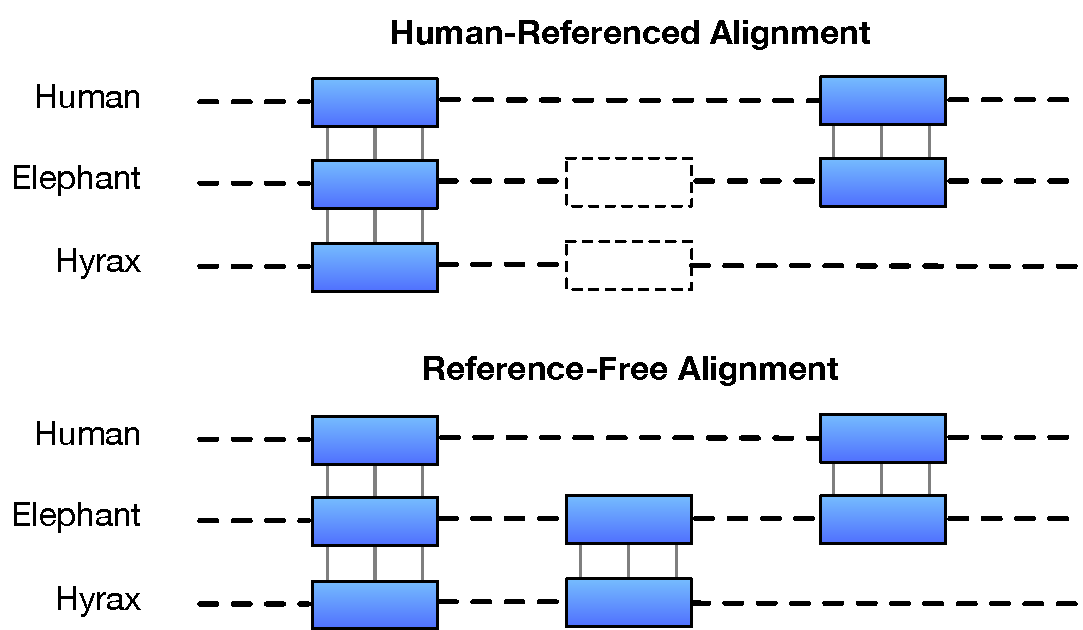
\includegraphics[width=0.75\textwidth]{reference-free-diagram}
\caption{A diagram showing the difference between a reference-free and a reference-biased multiple alignment. In a human-biased multiple alignment, any regions that are deleted in human, or inserted somewhere else in the tree, cannot be aligned.}\label{fig:referencefree}
\end{center}
\end{figure}

\begin{table}[ht]
\centering
\begin{tabular}{|l|l|p{12cm}|}
\hline
Program & Year & Description \\
\hline
ROSETTA & 2000 \cite{batzoglou2000human} & Uses pairwise genomic alignments to find regions of homology. Incorporates a splice junction and exon length model. \\
\hline
SGP-1/-2 & 2001 \cite{wiehe2001sgp} & Uses pairwise genomic alignments to find syntenic loci. Evaluates a coding and splice model in these loci.  \\
\hline
TWINSCAN & 2003 \cite{flicek2003leveraging} & Uses local alignments between a target genome and a reference (informant) genome to identify regions of conservation. \\
\hline
SLAM & 2003 \cite{alexandersson2003slam} & Treats two alignments in a symmetric way, predicting pairs of transcripts. \\
\hline
EvoGene & 2003 \cite{pedersen2003gene} & Phylogenetic HMM that performs \textit{ab-initio} prediction of genes across a multiple sequence alignment (more than 2 genomes), making use of phylogenetic information. \\
\hline
ExoniPhy & 2004 \cite{siepel2004computational} & Phylogenetic HMM that performs \textit{ab-initio} predictions across a multiple sequence alignment. \\
\hline
DOGFISH & 2006 \cite{carter2006vertebrate} & Two step program that combines a classifier that scores potential splice sites using a multiple sequence alignment and a \textit{ab-initio} gene predictor that makes use of the scores from the classifier to predict gene structures. \\
\hline
N-SCAN & 2006 \cite{gross2006using} & Extends the TWINSCAN model to $N$ genomes. \\
\hline
CONTRAST & 2007 \cite{gross2007contrast} & Uses a combination of SVM and CRF predictors, providing a big boost over traditional HMMs. \\
\hline
\end{tabular}
\caption{\label{tab:history}Overview of comparative annotation tools.}
\end{table}

\begin{table}[ht]
\centering
\begin{tabular}{|l|l|p{12cm}|}
\hline
Program & Year & Description \\
\hline
GeneWise & 2004 \cite{birney2004genewise} & HMM based gene prediction tool using extrinsic evidence. MAKER2 can make use of it. \\
\hline
NSCAN-EST & 2006 \cite{wei2006using} & HMM based gene prediction tool that makes use of EST and genomic alignments, incorporating phylogenetic information. \\
\hline
  AUGUSTUS & 2004 \cite{stanke2004augustus},\cite{stanke2006gene} & CRF based gene prediction tool with many modes. Features are still being added. Can perform \textit{ab-initio} gene prediction as well as incorporate extrinsic evidence. Has the ability to provide non-linear weights to various types of evidence. \\
\hline
EVM & 2008 \cite{haas2008automated,haas2013novo} & A `chooser' algorithm that combines previously predicted gene sets with extrinsic information to construct consensus gene sets. \\
\hline
PASA & 2003 \cite{haas2003improving} & Uses alignments of cDNA, EST or RNA-seq to predict gene structures, including alternative splice events. \\
\hline
MAKER2 & 2008 \cite{cantarel2008maker,yandell2012beginner} & A all-in-one pipeline that runs programs including AUGUSTUS and GeneWise with extrinsic information such as RNA-seq or protein sequences to both predict annotations and construct a gene set. \\
\hline
\end{tabular}
\caption{\label{tab:history_prediction}Overview of gene prediction tools that incorporate transcriptome data.}
\end{table}

\begin{table}[ht]
\centering
\begin{tabular}{|l|l|p{12cm}|}
\hline
Program & Year & Description \\
\hline
Projector & 2004 \cite{meyer2004gene} & Similar to DOUBLESCAN, but extends the model to make use of annotation information on one sequence to inform the other. Works better than GENEWISE over long branch lengths. \\
\hline
AIR & 2005 \cite{florea2005gene} & Integrates multiple forms of extrinsic evidence to perform alternative splice junction prediction. \\
\hline
transMap & 2007 \cite{stanke2008using} & Uses whole genome alignments to project existing annotations from one genome to one or more other genomes. \\
\hline
CESAR & 2016 \cite{sharma2016coding} & Uses a HMM to adjust splice sites in whole genome alignments, improving transcript projections. \\
\hline
\end{tabular}
\caption{\label{tab:history_comparative}Overview of transcript projection tools.}
\end{table}

\begin{table}[ht]
\begin{center}
\begin{tabular}{|l|l|p{12cm}|}
\hline
Program & Year & Description \\
\hline
Chains and nets & 2003~\cite{evoCauldron} & foo \\
\hline
\end{tabular}
\caption{\label{tab:pairwise_genome_alignment}Pairwise genome alignment tools.}
\end{center}
\end{table}

\begin{table}[ht]
\begin{center}
\begin{tabular}{|l|l|l|l|l|p{6cm}|}
\hline
Program & Year & Colinear & Reference-biased & Single-copy & Description \\
\hline
TBA & 2004~\cite{tba} & \checkmark & & \checkmark & Multiple aligner (using MultiZ internally) that produces a collection of partially ordered "threaded blocksets." \\
\hline
MultiZ (autoMZ) & 2004~\cite{tba} & & \checkmark & \checkmark & Multiple alignment based on pairwise alignment from every genome to a single reference. \\
\hline
ABA & 2004~\cite{aBruijn} & & & & Aligner based on the concept of A-Bruijn graphs. \\
\hline
% TODO(joel): original Mauve?
% TODO(joel): FSA? don't really feel like putting a bunch of colinear aligners in here.
EPO & 2008~\cite{epo, ortheus} & & * & & Graph-based aligner allowing duplications, and optionally producing ancestral reconstructions. \\
\hline
VISTA-Lagan (SuperMap) & 2009~\cite{vistaLagan} & * & & & Progressive aligner based on Shuffle-LAGAN \cite{shuffleLagan}. \\
\hline
progressiveMauve & 2010~\cite{progressivemauve} & & \checkmark & & Progressive aligner that attempts to remove anchors causing small rearrangements by optimizing a breakpoint-weighted score. \\
\hline
Cactus & 2011~\cite{cactusGenomeRes} & & & & Graph-based aligner that attempts to remove anchors representing small rearrangements. \\
\hline
\end{tabular}
\caption{\label{tab:multiple_genome_alignment}Multiple genome alignment tools.}
\end{center}
\end{table}

\clearpage
\bibliography{references}


\end{document}
